\textit{Response.} 

We begin by writing the most general form of a linear stochastic differential equation with multiplicative noise

\begin{equation}
	d \func{x}{t} = -\lambda\,\gpr{\func{x}{t} - \mu}\,dt + \func{\sigma}{t,\ \func{x}{t}}\,d \func{W}{t},
\end{equation}

where $\lambda > 0$ is real, and $\mu$ is the mean of the target distribution. For our case, $\mu = \frac{b + c}{2}$.

The Fokker-Planck equation gives a differential equation for the equilibrium distribution

\begin{equation}
	-\partial_{x} \gbkt{-\lambda\,\gpr{x - \mu}\,\func{p}{x}} + \frac{1}{2}\,\partial_x^2 \gbkt{\gpr{\func{\sigma}{x}}^2\,\func{p}{x}} = 0,
\end{equation}

where we have simply set $\partial_t p = 0$ in the time-dependent Fokker-Planck equation. To continue from here, we consider $\func{p}{x}$ as the limiting distribution of the following sequence of functions

\begin{equation}
	\func{\widetilde{p}}{x;\ n} = \frac{1}{c - b}\,e^{-\gpr{\frac{2}{c - b}\,\gpr{x - \frac{b + c}{2}}}^{2\,n}} = \frac{1}{c - b}\,e^{-y^{2\,n}},
\end{equation}

where we have used $y = \frac{2}{c - b}\,\gpr{x - \frac{b + c}{2}}$ for shorthand. Note that for $b < x < c$, we have $-1 < y < 1$, and so the limit $\lim_{n \to \infty} \func{\widetilde{p}}{x;\ n}$ is well-behaved except at the points $x = b$ and $x = c$, which we may ignore.\footnote{In particular, the limit is well-behaved on the disjoint open sets $\ointer{-\infty}{b}$, $\ointer{b}{c}$, and $\ointer{c}{\infty}$, and we may restrict our differential equation to these domains and manipulate it as we normally would.} We may thus rewrite the differential equation as

\begin{equation}
	-\partial_{x} \gbkt{-\lambda\,\gpr{x - \mu}\,\func{\widetilde{p}}{x;\ n}} + \frac{1}{2}\,\partial_x^2 \gbkt{\gpr{\func{\sigma}{x}}^2\,\func{\widetilde{p}}{x;\ n}} = 0
\end{equation}

and later take the limit $n \to \infty$. Integrating this equation once with respect to $x$, we obtain

\begin{equation}
	\lambda\,\gpr{x - \mu}\,\func{\widetilde{p}}{x;\ n} + \frac{1}{2}\,\dv{x} \gbkt{\gpr{\func{\sigma}{x}}^2\,\func{\widetilde{p}}{x;\ n}} = \text{const.} = 0,
\end{equation}

where $\text{const.} = 0$ as the probability distribution $\func{p}{x}$ (and its derivatives) must decay rapidly as $x \to -\infty$ and $x \to \infty$. The derivative of $\func{\widetilde{p}}{x;\ n}$ is given by

\begin{equation}
	\dv{\func{\widetilde{p}}{x;\ n}}{x} = -\frac{4\,n}{c - b}\,y^{2\,n-1}\,\func{\widetilde{p}}{x;\ n}.
\end{equation}

Therefore, the differential equation becomes

\begin{equation}
	\dv{x} \gbkt{\gpr{\func{\sigma}{x}}^2}\,\func{\widetilde{p}}{x;\ n} + \gpr{\func{\sigma}{x}}^2\,\gpr{-\frac{4\,n}{c - b}\,y^{2\,n-1}}\,\func{\widetilde{p}}{x;\ n} = 2\,\lambda\,\gpr{x - \mu}\,\func{\widetilde{p}}{x;\ n},
\end{equation}

For $\abs{y} > 1$, the limit as $n \to \infty$ of this differential equation becomes $0 + 0 = 0$ as $\func{\widetilde{p}}{x;\ n}$ decays faster than $\func{a}{x}$ and $\gpr{\func{\sigma}{x}}^2$. Thus, we only consider the case where $\abs{y} < 1$, in which the differential equation becomes

\begin{equation}
	\gpr{\abs{y} < 1}:\qquad \lim_{n \to \infty} \dv{x} \gbkt{\gpr{\func{\sigma}{x}}^2} + \gpr{\func{\sigma}{x}}^2\,\gpr{-\frac{4\,n}{c - b}\,y^{2\,n-1}} = \dv{x} \gbkt{\gpr{\func{\sigma}{x}}^2} = 2\,\lambda\,\gpr{x - \mu}.
\end{equation}

From which we may readily see that 

\begin{equation}
	\func{\sigma}{x} = \sqrt{\lambda\,\gpr{x^2 - 2\,\mu} + \mathcal{C}}
\end{equation}

where $\mathcal{C}$ is some constant, and we take only the positive square root as the variance is non-negative. We may determine the value of $\mathcal{C}$ by noting that $\func{\sigma}{b} = \func{\sigma}{c} = 0$, which fixes $\mathcal{C} = -\lambda\,b\,c$ Therefore, we have

\begin{equation}
	\func{\sigma}{x} = \sqrt{\lambda\,\gpr{x - b}\,\gpr{c - x}},
\end{equation}

as desired.

Below we include a plot of the euilibrium statistics across 1000 trials with $\lambda = 2$, $b = 1$, and $c = 5$, with a time-step size of $\Delta t = 0.05$. 

\begin{figure}[H]
	\centering
	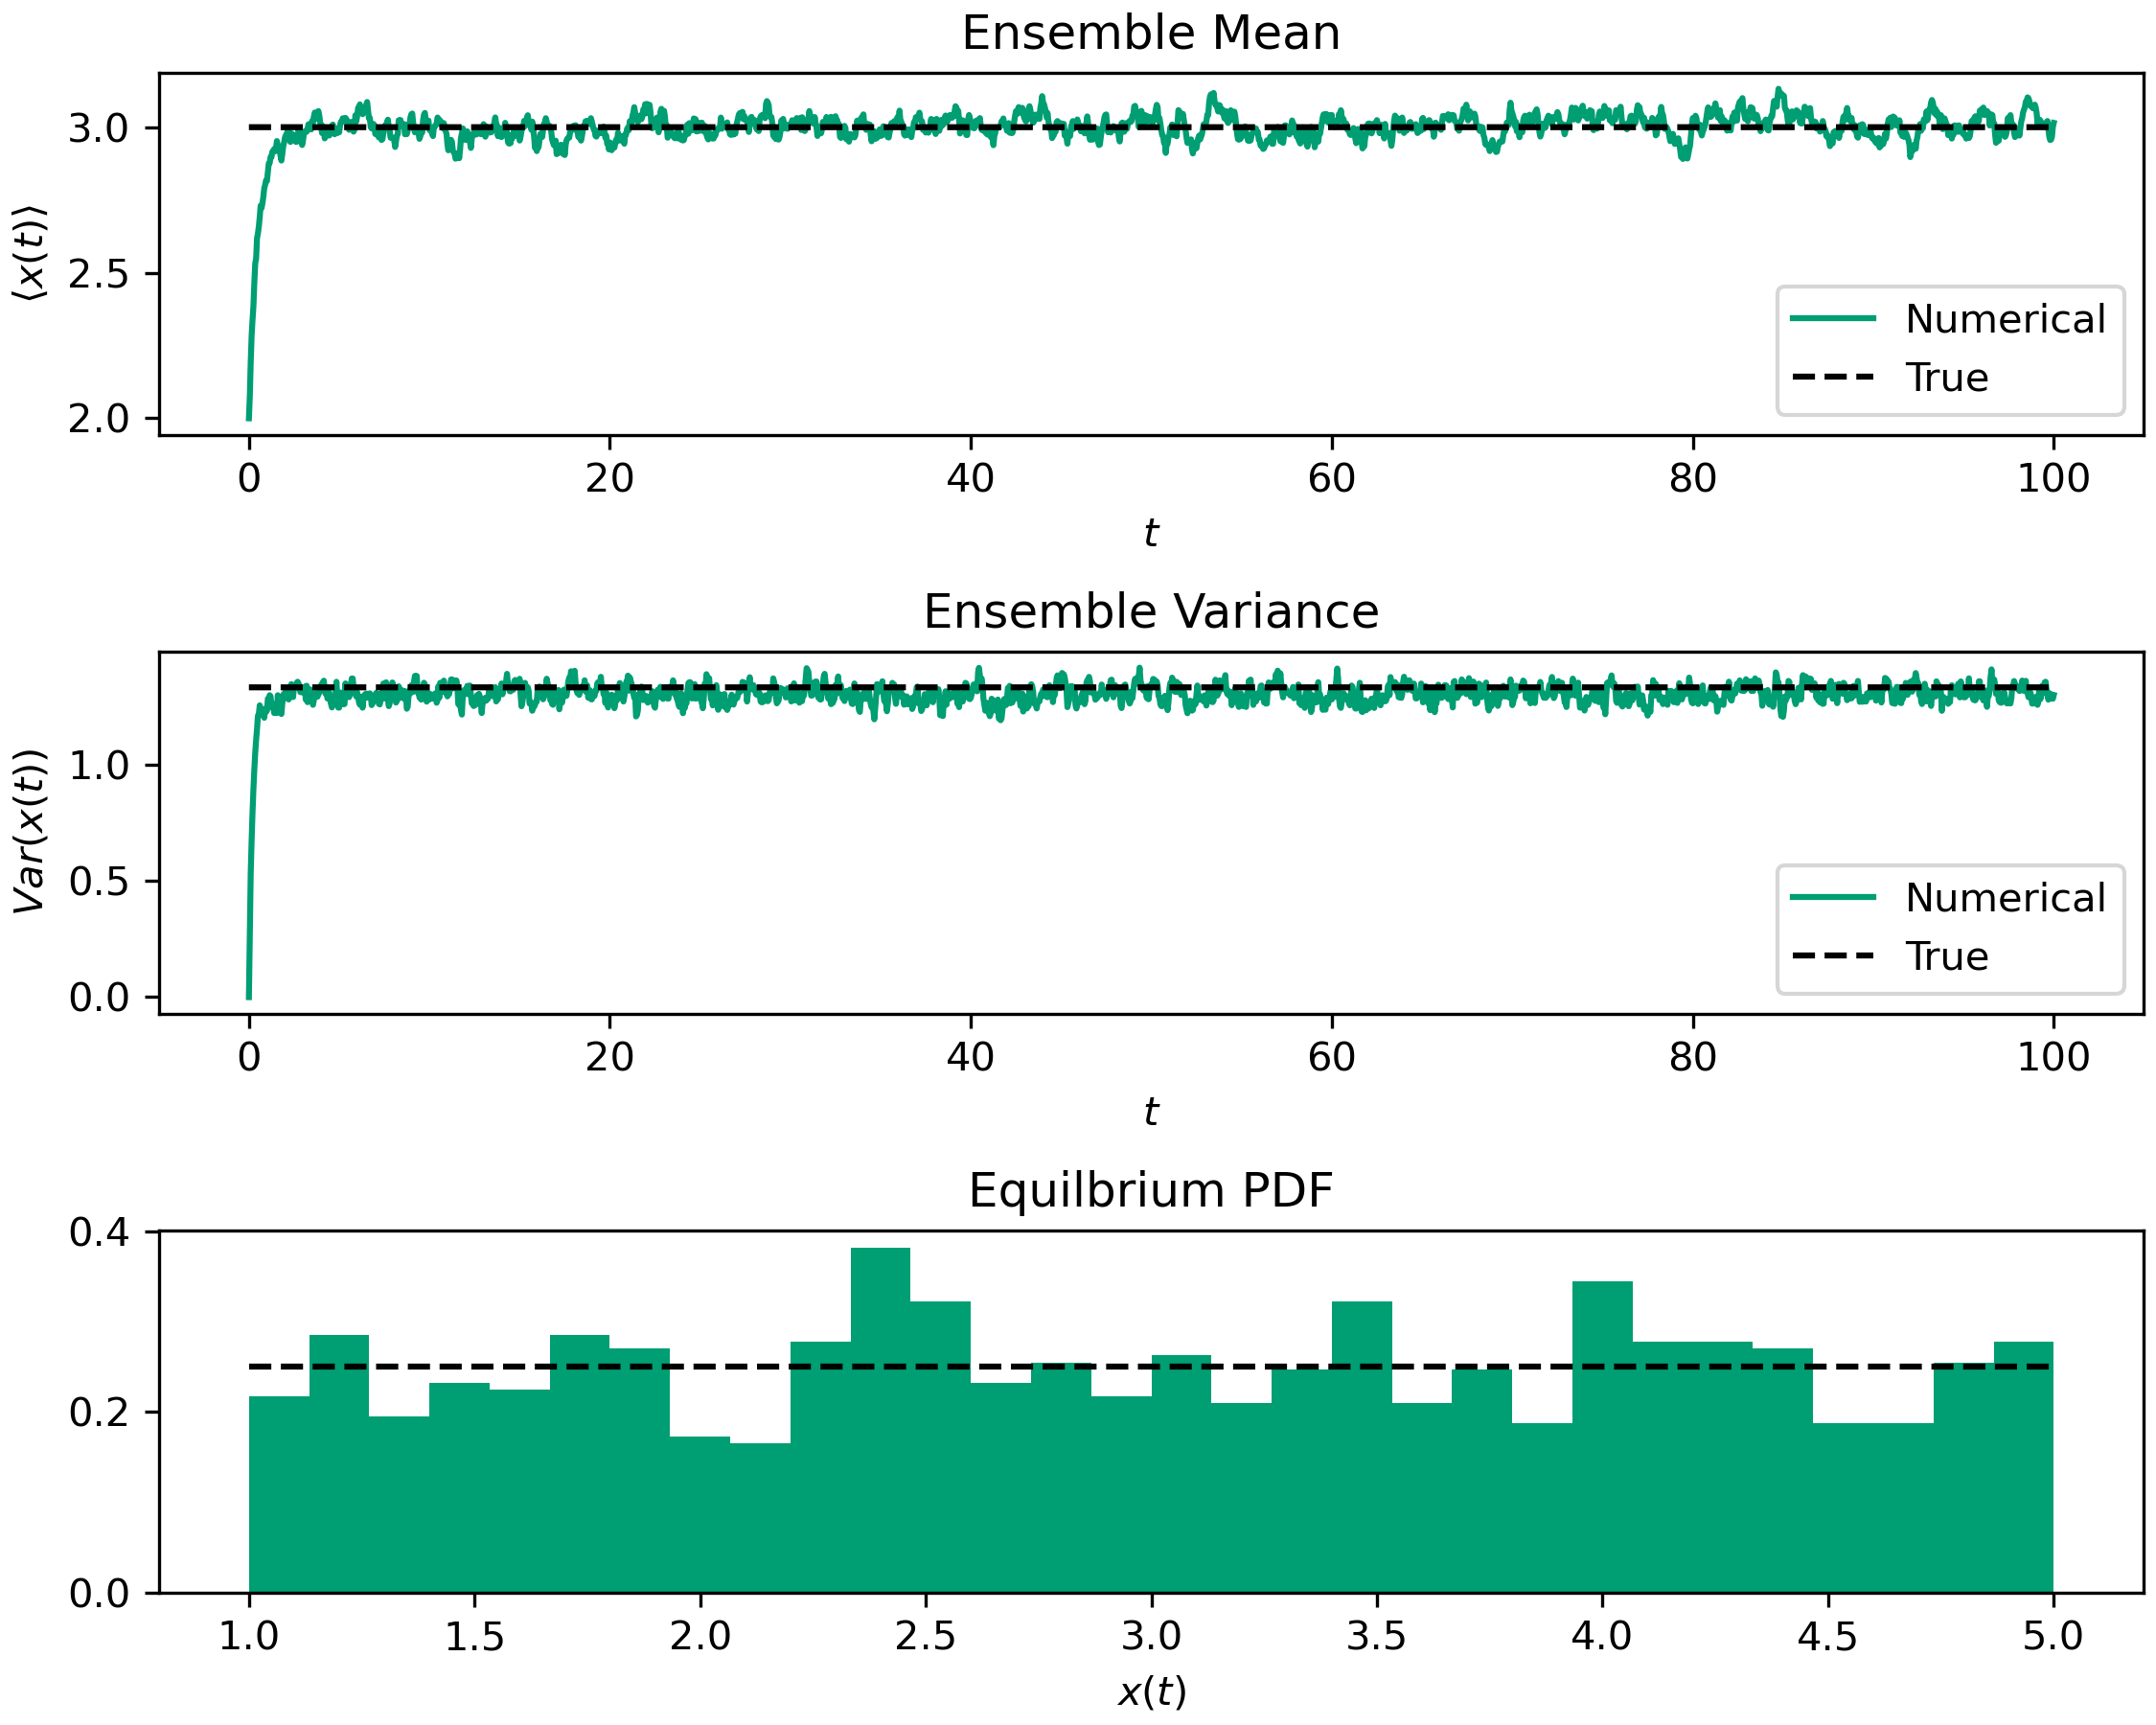
\includegraphics[width=0.75\textwidth]{../../src/1_ens_stats.png}
	\caption{The ensemble statistics for 1000 realizations of the linear SDE with multiplicative noise with the parameters $\lambda = 2$, $b = 1$, and $c = 5$ with initial condition $\frac{b + c}{3} = 2$ for each realization. The equilibrium values for the means and variances are given by the dashed horizontal black lines in the top two plots, and the true equilbirum distribution is given by the dashed horizontal black line in the bottom plot.}
	\label{fig:1_ens_stats}
\end{figure}

The SDE was discretized using the Euler--Maruyama scheme

\begin{equation}
	x_{k+1} = x_{k} - \lambda\,\gpr{x_{k} - \frac{b + c}{2}}\,\Delta t + \sqrt{\lambda\,\gpr{x_{k} - b}\,\gpr{c - x_{k}}}\,\sqrt{\Delta t}\,\xi_{k+1}
\end{equation}

where $\xi_{k+1}$ is sampled from a zero-mean unit-variance Gaussian distribution. If $x_{k+1} < b$, then we set $x_{k+1} = b$, and likewise for $x_{k+1} > c$. Source code is available from the GitHub repository
	
	\begin{center}
		\url{https://github.com/jasonltorchinsky/MATH833_HW/releases/tag/hw4}
	\end{center}

	and is given in Appendix~\ref{app:code_1}. In short, the code takes a input parameters \texttt{-l}, \texttt{-b}, and \texttt{-c} which correspond to $\lambda$, $b$, and $c$. The code then simulates 1000 individual realizations of the linear SDE with multiplicative noise using the Euler--Maruyama method, and plots a single trajectory along with the statistics across all 1000 realizations.
	

